\chapter{统计学}

\section{Learning Outcome}
Measure of Spread:
\begin{todolist}
\item 绘制频率直方图,累积频率直方图histogram\& cumulative frequency graph
\item 计算离散统计值的方差Variance和标准差Standard Deviation
\end{todolist}
\par

Probability:
\begin{todolist}
\item 一个事件概率的表示手段
\item 绘制tree diagram
\item 互斥事件mutually exclusive events与独立事件independent events的判断
\item 求算条件概率Conditional Probability
\end{todolist}
\par

Permutations \& Combinations:
\begin{todolist}
\item 阶乘factorial的表示方式和计算
\item 排列Permutation \& Arrangements的计算公式和应用
\item 组合Combination的计算公式以及应用
\item 插空法的使用
\end{todolist}
\par

Probability Distribution:
\begin{todolist}
\item 理解随机变量的含义,离散的和连续的Discrete and Continuous Random Variable
\item 计算随机变量的概率分布表Probability Distribution
\item 根据概率分布表,求算随机变量的期望Expectation和方差Variance
\end{todolist}
\clearpage

Binomial Distribution:
\begin{todolist}
\item 理解0-1分布实验
\item 理解二项分布Binomial Distribution实验,掌握表达方式,求算特定次数的概率,列出概率分布表
\item 求算二项分布的期望和方差
\item 理解几何分布Geometric Distribution实验,掌握表达方式,求算特定次数的概率,列出概率分布表
\item 求算几何分布的期望
\end{todolist}
\par

The Normal Distribution:
\begin{todolist}
\item 掌握正态分布表达方式,概率曲线形状,期望和标准差对概率曲线的影响,密度曲线包围的面积的意义
\item 对正态分布做标准化处理Standardize Normal Distribution
\item 能够从正态分布表查值
\item 利用标准正态分布解决相关的概率问题
\end{todolist}
\clearpage


\section{Key Concept}
\begin{enumerate}
\item 频率分布直方图histogram是将结果按照一定的interval统计频率绘制的图像。如下图所示:
\begin{figure}[H]
\centering
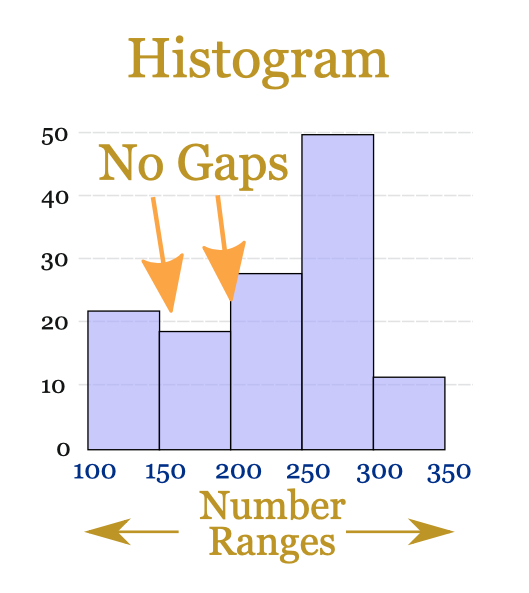
\includegraphics[width=200pt]{auximage/histogram.png}
\end{figure}
\item 累计频率分布表是将所有小于给定值的频率相加获取的,较大数值的累计频率必定大于等于较小数值的累计频率
\begin{table}[H]
\centering
\begin{tabular}{|c|c|c|c|}
\hline
$x$   & frequency & range         & cumulative frequency \\ \hline
10-20 & 4         & \textless{}20 & 4                    \\ \hline
20-30 & 9         & \textless{}30 & 13                   \\ \hline
30-35 & 7         & \textless{}40 & 20                   \\ \hline
35-50 & 3         & \textless{}50 & 23                   \\ \hline
\end{tabular}
\end{table}

\item 对于带有频率分布的统计值,求算\textcolor{r1}{平均值 Mean}的公式为:$\bar{x}=\frac{\sum x_i\cdot f_i}{\sum f_i}$。
\item 对于带有频率分布的统计值,求算\textcolor{r1}{方差 Variance}的公式为:\\
$Var(X)=\frac{\sum (x_i-\bar{x})^2\cdot f_i}{\sum f_i}=\frac{\sum x_i^2\cdot f_i}{\sum f_i}-\bar{x}^2$。

\textcolor{r1}{标准差 Standard Deviation}就是方差的正平方根。

\item 如果把一个事件记录为A,另外一个时间记录为B,那么$P(A)$表示A事件发生的概率,$P(A')$表示\textcolor{r1}{A的对立事件}发生的概率 $P(B)$表示B事件发生的概率,$P(AB)$或者$P(A\cap B)$或者$P(A and B)$表示AB同时发生的概率,而$P(A|B)$则表示在\textcolor{r1}{B事件已经发生}的条件下,A事件发生的概率。由于概率的定义,必定是介于0-1之间的一个数据。

\item tree diagram是将\textcolor{r1}{所有可能的结果}全部罗列出来的图表,并且在每一次的分支上可以记录发生的概率,沿着某一条路径分支一致走下去就是最终概率。并且所有分支的概率之和为1。一般考试节点级数不超过3个。如下图:\\
\begin{center}
\begin{tikzpicture}[grow=right, sloped]
\node[coin] {第一次}
    child {
        node[coin] {第二次}        
            child {
                node[end, label=right:
                    {$P_4=(1-p)\cdot(1-p)$}] {}
                edge from parent
                node[below]  {$1-p$}
            }
            child {
                node[end, label=right:
                    {$P_3=(1-p)\cdot p$}] {}
                edge from parent
                node[below]  {$p$}
            }
            edge from parent
            node[below]  {$1-p$}
    }
    child {
        node[coin] {第二次}        
        child {
                node[end, label=right:
                    {$P_2=p\cdot (1-p)$}] {}
                edge from parent
                node[below]  {$1-p$}
            }
            child {
                node[end, label=right:
                    {$P_1=p\cdot p$}] {}
                edge from parent
                node[below]  {$p$}
            }
        edge from parent
            node[below]  {$p$}
    };
\end{tikzpicture}
\end{center}

\item 两个事件为\textcolor{r1}{互斥事件Mutually Exclusive Events}是指这两个事件不能同时发生。因此$P(A\cap B)=0$

\item 两个事件为\textcolor{r1}{独立事件Independent Events是指两个事件没有任何联系。一个事件的发生不会影响第二个事件的发生与否}。因此$P(A\cap B)=P(A)\times P(B)$,或者说$P(A|B)=P(A)$, $P(B|A)=P(B)$

\item 条件概率\textcolor{r1}{Conditional Probability}就是指当某一个事件发生后,另一个事件发生的概率。有非常著名的贝叶斯公式。$P(A|B)=\frac{P(A\cap B)}{P(B)}$ 因此$P(A|B)\ge P(A)$

\item 阶乘factorial是一种正整数连乘的缩写手段,$n!=n\times (n-1)\times (n-2)\times \ldots\times 2\times 1$。其中通过阶乘的特殊性质,定义了$0!=1$
\item 排列是指从$n$个物体当中,取出$r$个物体,并且按照特定的顺序将这个$r$个物体进行排列,记录有多少种不同的排列顺序。比如学生站队的问题。那我们直接通过Permutation的求算。$^nP_r=\frac{n!}{(n-r)!}$。核心关键词是\textcolor{r1}{Arrange,align}
\item 组合是指从$n$个物体当中,取出$r$个物体,而无需考虑这$r$个物体的先后顺序,记录所有可行的抽选方案数目。可以直接通过Combination的公式进行求算$^nC_r=\frac{^nP_r}{r!}=\frac{n!}{(n-r)!\cdot r!}$,可以认为是对应Permutation,除以$r!$种重复顺序得来的。另外一种标记手段是$n\choose r$,在二项分布和二项展开式当中这种形式居多。

\item 插空法是常用的解题方法,通常用于多个物体必须要\textcolor{r1}{紧密相邻},或者多个物体\textcolor{r1}{不能相邻}的情况。其思路是:

a. 将没有做其他要求的剩余物体进行Permutation;\\
b. 数出有多少个空隙,记为$n$;\\
c-1. 如果要求是$r$个物体相邻,则将这r个物体进行Permutaion,再任选空隙当中的一个进行插入$r! \cdot{n \choose 1}$;\\
c-2. 如果要求是$r$个物体不能相邻,则从空隙当中选择出$r$个空,再\textcolor{r1}{有顺序地}将物体插入至空隙中;因此结果为${n\choose r} \cdot r!$或者直接用$^nP_r$.\\
d. 最后利用\textcolor{r1}{乘法法则}求算最终结果
\item 随机变量Random Variable,一般用大写字母$X$表示,代表着某一个试验最终所有可能的结果。这里由于并没有真正去做这次实验,因此我们是从假设预估的角度上进行探究的。而离散的随机变量指X的取值为离散数值,一般为\textcolor{r1}{整数}。连续随机变量则是指X能取到\textcolor{r1}{所有实数值}

\item 离散随机变量的概率分布表就是如下图所示的一张表:

\begin{table}[H]
\centering
\begin{tabular}{|l|c|c|c|c|}
\hline
$X$    & $x_1 $& $x_2$  & $x_3$ & $x_4$ \\ \hline
$P(X)$ & $p_1$ & $p_2$ & $p_3$ & $p_4$ \\ \hline
\end{tabular}
\end{table}

其中$x_i$是随机变量X的取值,下方则表示对应的概率。有一个很重要的性质经常会用于解题当中,由于这张表是所有可能取值,因此\textcolor{r1}{把所有概率加起来最后结果等于1}。在考试当中基本上不会给表格,而是给出概率随取值的函数关系$P(x=k)=f(k)$,要能够理解这种函数关系,并且转化到这张表

\item 从概率分布表,可以求算该随机变量的\textcolor{r1}{期望和方差},需要牢记公式:

期望Expectation $E(X)=\sum x_i\cdot P(x_i)$

方差Variance $Var(X)=\sum (x_i-E(X))^2\cdot P(x_i)$

\item 0-1分布指随机试验的结果只有两种的分布情况,可以用0代表失败,用1代表成功。最为经典的例子为抛硬币。0-1分布的表格为:

\begin{table}[H]
\centering
\begin{tabular}{|l|c|c|}
\hline
$X$    & $0$   & $1$ \\ \hline
$P(X)$ & $1-p$ & $p$ \\ \hline
\end{tabular}
\end{table}

\item 二项分布实验Binomial Distribution,则是将0-1分布实验\textcolor{r1}{重复执行$n$次}。用随机变量$X$来表示在这$n$次实验当中\textcolor{r1}{成功的次数}。表达方式为为$X\sim B(n,p)$。其中具有两个\textcolor{r1}{参数parameter},实验重复次数$n$以及单次成功的概率$p$。由于每次实验之间都是互相独立的,因此如果成功次数为$k$的话,概率为$P(X=k)= {n\choose k} \cdot p^k\cdot (1-p)^{n-k}$。

\begin{table}[H]
\centering
\begin{tabular}{|l|c|c|c|c|c|c|c|}
\hline
$X$    & $0$       & $1$                                                  & $\ldots$ & $k$                         & $\ldots$ & $n$   \\ \hline
$P(X)$ & $(1-p)^n$ & ${n\choose 1} p^1(1-p)^{n-1}$  & $\ldots$ & ${n\choose k} p^k(1-p)^{n-k}$ & $\ldots$ & $p^n$ \\ \hline
\end{tabular}
\end{table}

\item 因此使用该概率分布表,可以求算二项分布的期望和方差,分别为$E(X)=np$,$Var(X)=np(1-p)$。这两个公式\textcolor{r1}{无需证明},只需要运用即可。

\item 几何分布Geometric Distribution也是从0-1分布演变而来的,但是和二项分布不一样的是,在几何分布实验中,并不是指定做多少次实验,而是要\textcolor{r1}{一直重复做0-1实验,直到成功}。再用随机变量$X$表示总共需要的次数。计作$X\sim Geo(p)$。其中只有一个\textcolor{r1}{参数,成功的概率$p$}。比如$X=3$意味着前两次失败,第三次成功。因此求算几何分布的概率分布表则如下表所示

\begin{table}[H]
\centering
\begin{tabular}{|l|c|c|c|l|l|}
\hline
$X$    & $1$ & $2$      & $\ldots$ & $k$              & $\ldots$ \\ \hline
$P(X)$ & $p$ & $(1-p)p$ & $\ldots$ & $(1-p)^{k-1}\cdot p$ & $\ldots$ \\ \hline
\end{tabular}
\end{table}

几何分布和二项分布最不一样的地方在于这个概率分布表\textcolor{r1}{从1开始,并且无穷无尽}。而且不管$X$取值为多少,只能是在最后一次成功

\item 仅考察几何分布的\textcolor{r1}{期望},求算公式为$E(X)=\frac{1}{p}$

\item 正态分布Normal Distribution是最为重要的\textcolor{r1}{连续}分布,也是日常生活当中非常常见的分布情况。不需要掌握正态分布的概率密度函数,仅需要记住正态分布的\textcolor{r1}{图像}如下图所示:

\begin{tikzpicture}
\begin{axis}[
  no markers, domain=-5:10, samples=200,
  axis lines*=left, xlabel=$x$, ylabel=$y$,
  every axis y label/.style={at=(current axis.above origin),anchor=south},
  every axis x label/.style={at=(current axis.right of origin),anchor=west},
  height=5cm, width=12cm,      %图像的大小
  xtick={-1,0,4}, ytick=\empty,  %tick标记手段只能用集合的方式
  enlargelimits=false, clip=false, axis on top,
  grid = major
  ]
  %\addplot [fill=cyan!20, draw=none, domain=0:5.96] {gauss(6.5,1)} \closedcycle; 标记面积的
  \addplot [very thick,r1!50] {gauss(4,2)};
  \addplot [very thick,b1!50] {gauss(-1,3)};
  \addplot [very thick,p1!50] {gauss(0,1)};
\end{axis}
\end{tikzpicture}

\item 对于服从正态分布的随机变量,我们的标记手段为,$X\sim N(\mu, \sigma^2)$。其中,$\mu$为正态分布的期望,$\sigma$代表标准差standard deviation。从上图当中,可以看出任意正态分布的曲线都是类似的,但是$\mu$会使分布图像水平移动,$\sigma$则会使图像发生竖直方向的拉伸变形。并且特征是,当$\sigma$越大的时候,分布更加的分散,因此会压扁函数图像。

上图的三个正态分布,分别为$N(0,1^2)$,$N(4,2^2)$,$N(-1,3^2)$。尝试区分对应关系

\item 对于正态分布的图像,最重要的是\textcolor{r1}{图像下方包围的面积}

\begin{tikzpicture}
\begin{axis}[
  no markers, domain=0:10, samples=200, 
  axis lines*=left, xlabel=$x$, ylabel=$\phi(x)$,
  every axis y label/.style={at=(current axis.above origin),anchor=south},
  every axis x label/.style={at=(current axis.right of origin),anchor=west},
  height=5cm, width=12cm,      %图像的大小
  xtick=\empty, ytick=\empty,  %tick标记手段
  enlargelimits=false, clip=false, axis on top,
  grid = major
  ]
  \addplot [fill=r1!20, draw=none, domain=1:7] {gauss(4,1)} \closedcycle; 
  \addplot [fill=b1!20, draw=none, domain=2:6] {gauss(4,1)} \closedcycle; 
  \addplot [fill=p1!20, draw=none, domain=3:5] {gauss(4,1)} \closedcycle; 
  \addplot [very thick,p1!50] {gauss(4,1)};
  \draw [yshift=-0.3cm, latex-latex](axis cs:3,0) -- node [fill=white] {$\mu\pm\sigma$} (axis cs:5,0);
  \draw [yshift=-0.8cm, latex-latex](axis cs:2,0) -- node [fill=white] {$\mu\pm 2\sigma$} (axis cs:6,0);
  \draw [yshift=-1.4cm, latex-latex](axis cs:1,0) -- node [fill=white] {$\mu\pm3\sigma$} (axis cs:7,0);
\end{axis}
\end{tikzpicture}

上图所示,阴影部分面积分别表示随机变量的取值在偏离期望1个标准差, 2个标准差,以及3个标准差的的概率大小。$P(\mu-\sigma <X<\mu+\sigma)=68.3\%$,$P(\mu-2\sigma <X<\mu+2\sigma)=95.4\%$,$P(\mu-3\sigma <X<\mu+3\sigma)=99.7\%$
这个关系对于任意的正态分布总是成立的。


\item 既然所有的正态分布都可以通过拉伸变形到同样的图像,我们选择$N(0,1^2)$的正态分布作为这个基本图像,称之为\textcolor{r1}{标准正态分布Standard Normal Distribution},那么其他任意分布都可以通过移动和变形回到标准正态分布的曲线上。这个过程叫做标准化Standardization。

假设$X\sim N(\mu,\sigma^2)$,那么引入新的随机变量$Z$,使$Z=\frac{X-\mu}{\sigma}$,这个随机变量$Z$会服从标准正态分布。$Z\sim N(0,1^2)$。因此$P(X>k)$就完全等价于$P(Z>\frac{k-\mu}{\sigma})$,到标准正态分布表里去找值就好了。
\clearpage



\item 标准正态分布表是如下图的一张表,是求算$N(0,1^2)$分布中,随机变量小于$z$值的概率。$\Phi(z)=P(X<z)=\int_{-\infty}^{z} N(0,1^2) \d x=\int_{-\infty}^{z} \phi(x) \d x$:

\begin{tikzpicture}
\centering
\begin{axis}[
  no markers, domain=-4:4, samples=200, 
  axis lines*=left, xlabel=$x$, ylabel=$\phi(x)$,
  every axis y label/.style={at=(current axis.above origin),anchor=south},
  every axis x label/.style={at=(current axis.right of origin),anchor=west},
  height=5cm, width=12cm,      %图像的大小
  xtick={0,2.04}, ytick=\empty,  %tick标记手段
  enlargelimits=false, clip=false, axis on top,
  grid = major
  ]
  \addplot [fill=r1!20, draw=none, domain=-4:2.04] {gauss(0,1)} \closedcycle; 
  \addplot [very thick,r1!50] {gauss(0,1)};
\end{axis}
  \node [below] at (8,1) {$z$};
\end{tikzpicture}

\begin{longtable}{|r|rrrrrrrrrr|}
  \hline
 & 0.00 & 0.01 & 0.02 & 0.03 & 0.04 & 0.05 & 0.06 & 0.07 & 0.08 & 0.09 \\ 
  \hline
0.0 & 0.5000 & 0.5040 & 0.5080 & 0.5120 & 0.5160 & 0.5199 & 0.5239 & 0.5279 & 0.5319 & 0.5359 \\ 
  0.1 & 0.5398 & 0.5438 & 0.5478 & 0.5517 & 0.5557 & 0.5596 & 0.5636 & 0.5675 & 0.5714 & 0.5753 \\ 
  0.2 & 0.5793 & 0.5832 & 0.5871 & 0.5910 & 0.5948 & 0.5987 & 0.6026 & 0.6064 & 0.6103 & 0.6141 \\ 
  0.3 & 0.6179 & 0.6217 & 0.6255 & 0.6293 & 0.6331 & 0.6368 & 0.6406 & 0.6443 & 0.6480 & 0.6517 \\ 
  0.4 & 0.6554 & 0.6591 & 0.6628 & 0.6664 & 0.6700 & 0.6736 & 0.6772 & 0.6808 & 0.6844 & 0.6879 \\ 
  0.5 & 0.6915 & 0.6950 & 0.6985 & 0.7019 & 0.7054 & 0.7088 & 0.7123 & 0.7157 & 0.7190 & 0.7224 \\ 
  0.6 & 0.7257 & 0.7291 & 0.7324 & 0.7357 & 0.7389 & 0.7422 & 0.7454 & 0.7486 & 0.7517 & 0.7549 \\ 
  0.7 & 0.7580 & 0.7611 & 0.7642 & 0.7673 & 0.7704 & 0.7734 & 0.7764 & 0.7794 & 0.7823 & 0.7852 \\ 
  0.8 & 0.7881 & 0.7910 & 0.7939 & 0.7967 & 0.7995 & 0.8023 & 0.8051 & 0.8078 & 0.8106 & 0.8133 \\ 
  0.9 & 0.8159 & 0.8186 & 0.8212 & 0.8238 & 0.8264 & 0.8289 & 0.8315 & 0.8340 & 0.8365 & 0.8389 \\ 
  1.0 & 0.8413 & 0.8438 & 0.8461 & 0.8485 & 0.8508 & 0.8531 & 0.8554 & 0.8577 & 0.8599 & 0.8621 \\ 
  1.1 & 0.8643 & 0.8665 & 0.8686 & 0.8708 & 0.8729 & 0.8749 & 0.8770 & 0.8790 & 0.8810 & 0.8830 \\ 
  1.2 & 0.8849 & 0.8869 & 0.8888 & 0.8907 & 0.8925 & 0.8944 & 0.8962 & 0.8980 & 0.8997 & 0.9015 \\ 
  1.3 & 0.9032 & 0.9049 & 0.9066 & 0.9082 & 0.9099 & 0.9115 & 0.9131 & 0.9147 & 0.9162 & 0.9177 \\ 
  1.4 & 0.9192 & 0.9207 & 0.9222 & 0.9236 & 0.9251 & 0.9265 & 0.9279 & 0.9292 & 0.9306 & 0.9319 \\ 
  1.5 & 0.9332 & 0.9345 & 0.9357 & 0.9370 & 0.9382 & 0.9394 & 0.9406 & 0.9418 & 0.9429 & 0.9441 \\ 
  1.6 & 0.9452 & 0.9463 & 0.9474 & 0.9484 & 0.9495 & 0.9505 & 0.9515 & 0.9525 & 0.9535 & 0.9545 \\ 
  1.7 & 0.9554 & 0.9564 & 0.9573 & 0.9582 & 0.9591 & 0.9599 & 0.9608 & 0.9616 & 0.9625 & 0.9633 \\ 
  1.8 & 0.9641 & 0.9649 & 0.9656 & 0.9664 & 0.9671 & 0.9678 & 0.9686 & 0.9693 & 0.9699 & 0.9706 \\ 
  1.9 & 0.9713 & 0.9719 & 0.9726 & 0.9732 & 0.9738 & 0.9744 & 0.9750 & 0.9756 & 0.9761 & 0.9767 \\ 
  2.0 & 0.9772 & 0.9778 & 0.9783 & 0.9788 & \fcolorbox{red}{white}{0.9793} & 0.9798 & 0.9803 & 0.9808 & 0.9812 & 0.9817 \\ 
  2.1 & 0.9821 & 0.9826 & 0.9830 & 0.9834 & 0.9838 & 0.9842 & 0.9846 & 0.9850 & 0.9854 & 0.9857 \\ 
  2.2 & 0.9861 & 0.9864 & 0.9868 & 0.9871 & 0.9875 & 0.9878 & 0.9881 & 0.9884 & 0.9887 & 0.9890 \\ 
  2.3 & 0.9893 & 0.9896 & 0.9898 & 0.9901 & 0.9904 & 0.9906 & 0.9909 & 0.9911 & 0.9913 & 0.9916 \\ 
  2.4 & 0.9918 & 0.9920 & 0.9922 & 0.9925 & 0.9927 & 0.9929 & 0.9931 & 0.9932 & 0.9934 & 0.9936 \\ 
  2.5 & 0.9938 & 0.9940 & 0.9941 & 0.9943 & 0.9945 & 0.9946 & 0.9948 & 0.9949 & 0.9951 & 0.9952 \\ 
  2.6 & 0.9953 & 0.9955 & 0.9956 & 0.9957 & 0.9959 & 0.9960 & 0.9961 & 0.9962 & 0.9963 & 0.9964 \\ 
  2.7 & 0.9965 & 0.9966 & 0.9967 & 0.9968 & 0.9969 & 0.9970 & 0.9971 & 0.9972 & 0.9973 & 0.9974 \\ 
  2.8 & 0.9974 & 0.9975 & 0.9976 & 0.9977 & 0.9977 & 0.9978 & 0.9979 & 0.9979 & 0.9980 & 0.9981 \\ 
  2.9 & 0.9981 & 0.9982 & 0.9982 & 0.9983 & 0.9984 & 0.9984 & 0.9985 & 0.9985 & 0.9986 & 0.9986 \\ 
  3.0 & 0.9987 & 0.9987 & 0.9987 & 0.9988 & 0.9988 & 0.9989 & 0.9989 & 0.9989 & 0.9990 & 0.9990 \\ 
   \hline
\end{longtable}
使用这张表的过程是比较简单的,比如查找$\Phi(2.04)$直接先搜寻第一排竖排$2.0$,再水平移动至第五个,选择$0.04$这一栏。找出交点数值为0.9788。就表示在$N(0,1^2)$分布中,随机变量小于$2.04$的概率为0.9793。考试当中也可能反向查找,比如给定概率为0.9788寻找对应的$z$值。

\end{enumerate}
\end{document}